\documentclass[mathserif]{beamer} % Al parecer la indicacion mathserif le dice que la parte matematica va a ser con serif

\usepackage[orientation=portrait,size=a0,scale=1.4,debug]{beamerposter}
%\usepackage{epstopdf}

\mode<presentation>
    {
      \usepackage{styles/beamerthemeFEV}
    }
    \usepackage[scaled]{helvet} % letra principal no es serif es la letra helvetica

    \usepackage[cm]{mathdesign} % letra de la parte matemática: tipo charter

    \usepackage{amsmath,amsthm, amssymb, latexsym}

    %\usepackage[spanish,activeacute]{babel}
    \usepackage{graphicx} % funcionalidad extra al incluir graficos
    \usepackage[utf8]{inputenc} 


    \usepackage{ragged2e}
    \usepackage{subfigure}

    \usepackage{graphicx}

    \usepackage{textpos} % para poner bloques de texto en ubicaciones determinadas?

    \usepackage{fix-cm}
    \newcommand{\vect}[1]{\vec{\mathbf{#1}}}
    \newcommand{\vers}[1]{\breve{\mathbf{#1}}}
    \newcommand{\amp}[1]{\hat{#1}}
    \newcommand{\tensor}[1]{\overline{\overline{\mathbf{#1}}}}
    \newcommand{\matriz}[1]{\mathbf{#1}}
    \newcommand{\dist}[2]{\overline{#1 #2}} % distancia
    \newcommand{\hl}[1]{\colorbox{yellow}{#1}}
    \newcommand{\estim}[1]{\widehat{#1}} % estimado estimación

    %\date{26 de Agosto de 2014}
    \title[] % (optional, use only with long paper titles)
          {Diseño de un controlador de un actuador electrodinámico aplicado a interferometría dinámica}
          \author[Roman Zarza Verstraeten Riobo Veiras]{{\normalsize Santiago Roman \and Ezequiel M. Zarza \and Federico Verstraeten \inst{1} \\ Lucas M. Riobó \inst{1,2} \and Francisco E. Veiras \inst{1,2,3}}} 
          \institute[GLOMAE]{\centering {\it\footnotesize{ \inst{1} GLOmAe,
                Dpto. Física, Universidad de Buenos Aires \vspace{-2ex} \and
                \inst{2} CONICET, Buenos Aires \vspace{-2ex} \and \inst{3} INTI,
                Electrónica e Informática \vspace{-2ex} \and -}}}

          \begin{document}

          \begin{frame}

            \begin{columns}[T]
              \begin{column}{.475\linewidth}
                \vspace{-2ex}
                \begin{block}{Resumen}
                  \justifying
                  Un actuador es un dispositivo capaz de transformar energía (eléctrica para nuestro caso de interés) en la activación de un proceso, con la finalidad de generar un efecto sobre un proceso automatizado. Al mismo tiempo, existe un controlador encargado de enviar órdenes al actuador, con las cuales se activa un elemento final de control.
                  En este proyecto se busca diseñar un actuador electrodinámico, que se utilizará en un esquema interferométrico como el de Michelson.
                      \begin{center}
                        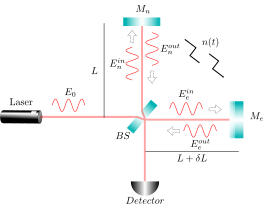
\includegraphics[width=1\linewidth]{img/michelson.pdf}
                      \end{center}
                       \justifying
                      
Para ello, valiendose de una fuente $laser$, se coloca un divisor de haz que divide y luego superpone dos campos eléctricos provenientes de la fuente. El campo que se desvía hacia la rama superior se refleja mediante un espejo fijo ($M_n$) mientras que el campo que se desvía hacia la derecha se refleja en un espejo móvil ($M_e$). De esta manera, los campos reflejados se dirigen hacia la rama inferior, donde se superponen en un fotodetector por medio del cual se puede registrar la intensidad de estos dos campos superpuestos.
      \end{block}
                 \vspace{-2ex}
                \begin{block}{Demodulación de fase}
                \justifying
   Reemplazando el espejo fijo $M_n$ por uno móvil, el esquema interferométrico modificará la señal de salida de manera tal que aparece una señal portadora y una moduladora (Modulación AM) , como se muestra a continuación.
Desfasaje continuo:
                      \begin{center}
                        \includegraphics[width=0.9\linewidth]{img/desfasaje_continuo.pdf}
                      \end{center}
                   11   \vspace{-1ex}
Desfasaje discreto:
\begin{center}
                        \includegraphics[width=0.9\linewidth]{img/desfasaje_discreto.pdf}
                      \end{center}
                  \justifying
                  donde $L_1$, $L_2$ y $\delta L$ representan diferentes caminos ópticos, y $\lambda_0$ es la longitud de onda del haz incidente. De esta manera, con la ayuda del fotodetector se puede medir la intensidad producida por la diferencia de camino óptico ($\delta L$).
                \end{block} 
                \vspace{-2ex}
                
              \end{column}

              \begin{column}{.475\linewidth}
                \vspace{-2ex}
	\begin{block}{Moduladores de fase: Nuestra propuesta}  
               \justifying
               Se utilizará un espejo a un parlante acoplado, como medio para introducir un desfasaje en una de las ramas del interferómetro. Para ello, el parlante estará controlado por un microcontrolador.\\
                  Colocando el parlante en una de las ramas del sistema interferométrico (ver imágenes adjuntas), se puede modular la diferencia de camino óptico del haz que incide sobre el espejo móvil, conectado al microcontrolador. \\
Es decir, el objetivo del parlante es poder lograr introducir una diferencia de camino optico (un desfasaje) controlado por medio de una señal de control. Esto podría permitir, que controlando la posición del espejo se pueden determinar la longitud de onda de la fuente lumínica y los parámetros $A$ y $B$ explicados anteriormente.

                  \vspace{1ex}

                  \begin{columns}
                    \begin{column}{.33\linewidth}
                      \begin{center}
                        \includegraphics[width=0.8\linewidth]{img/interferometro1.png}
                      \end{center}
                    \end{column} 
                    \begin{column}{.33\linewidth}
                      \begin{center}
                        \includegraphics[width=0.8\linewidth]{img/interferometro3.png}
                      \end{center}
                    \end{column}
            
            \begin{column}{.33\linewidth}
            	\begin{center}
                \includegraphics[width=0.8\linewidth] {img/parlante_espejov2.png}
                 \end{center}
                 \end{column}

				\end{columns}
                \end{block}
                \vspace{1ex}
                
                \vspace{-2ex}

                \begin{block}{Consideraciones de diseño e implementación}
			\justifying
             El microcontrolador puede recibir o establecer el tipo de desplazamiento que se aplicará sobre el parlante mediante transconductancia eléctrica-mecánica. Dicho modo de desplazamiento puede ser recibido mediante la interfaz USB/Serie que vincula al microcontrolador con la PC, como también ser seleccionado a través de un teclado (pulsadores) conectado al microcontrolador, donde el usuario elegirá el tipo de desplazamiento a realizar mediante las opciones vistas en el display, y será el microcontrolador el encargado de efectuarlas, a diferencia de la otra forma, donde solo actuará como intermediario.
                      \begin{center}
                        \includegraphics[width=0.9\linewidth]{img/diagrama_de_bloques.pdf}
                      \end{center}
                \end{block}

                \vspace{-3ex}
                \begin{block}{Conclusiones}
                  \justifying
El presente proyecto es llevado a cabo en el marco de las materias "Laboratorio de Microcomputadoras" (66.08) y "Laboratorio de Microprocesadores" (86.07) de la carrera de Ingeniería Electrónica (FIUBA).\\
Agradecemos a los docentes de la materia, quienes aportan pautas y lineamientos para el desarrollo del proyecto durante las clases; y a los miembros del equipo del GLOmAe brindando apoyo, prestando las instalaciones e instrumental, y colaborando con las tareas de mediciones y calibración del dispositivo. \\
Los próximos pasos serán continuar con el armado, puesta a punto y calibración del dispositivo en desarrollo. \\
A futuro se pretende que el dispositivo permita estabilizar el interferómetro, logrando eliminar las variaciones de fase en las ramas ópticas. Para ello se deberá desarrollar un sistema retroalimentado que permita medir esas variaciones a intervalos de tiempo, y corregir según corresponda.

                \end{block}


              \end{column}

            \end{columns} 

          \end{frame}

          \end{document}
